\documentclass[]{jarticle}          % 一段組
%\documentclass[twocolumn]{jarticle} % 二段組

\textwidth 180mm
\textheight 255mm
\oddsidemargin -12mm
\topmargin -15mm
\columnsep 10mm

%\vspace{0.5cm} % 一段組の場合はコメントアウトした方が体裁がよいx
%] % 一段組の場合はコメントアウトする

\usepackage{styles/labheadings}
\usepackage[dvipdfmx]{graphicx,color}
\usepackage{amsmath,amssymb}
\usepackage{url}
% 追加
\usepackage{listings,jvlisting}
\usepackage[hang,small,bf]{caption}
\usepackage[subrefformat=parens]{subcaption}
\captionsetup{compatibility=false}

\newcommand{\aU}{\mbox{\boldmath $a$}}
\newcommand{\bU}{\mbox{\boldmath $b$}}
\newcommand{\cU}{\mbox{\boldmath $c$}}
\newcommand{\dU}{\mbox{\boldmath $d$}}
\newcommand{\eU}{\mbox{\boldmath $e$}}
\newcommand{\fU}{\mbox{\boldmath $f$}}
\newcommand{\gU}{\mbox{\boldmath $g$}}
\newcommand{\hU}{\mbox{\boldmath $h$}}
\newcommand{\iU}{\mbox{\boldmath $i$}}
\newcommand{\jU}{\mbox{\boldmath $j$}}
\newcommand{\kU}{\mbox{\boldmath $k$}}
\newcommand{\lU}{\mbox{\boldmath $l$}}
\newcommand{\mU}{\mbox{\boldmath $m$}}
\newcommand{\nU}{\mbox{\boldmath $n$}}
\newcommand{\oU}{\mbox{\boldmath $o$}}
\newcommand{\pU}{\mbox{\boldmath $p$}}
\newcommand{\qU}{\mbox{\boldmath $q$}}
\newcommand{\rU}{\mbox{\boldmath $r$}}
\newcommand{\sU}{\mbox{\boldmath $s$}}
\newcommand{\tU}{\mbox{\boldmath $t$}}
\newcommand{\uU}{\mbox{\boldmath $u$}}
\newcommand{\vU}{\mbox{\boldmath $v$}}
\newcommand{\wU}{\mbox{\boldmath $w$}}
\newcommand{\xU}{\mbox{\boldmath $x$}}
\newcommand{\yU}{\mbox{\boldmath $y$}}
\newcommand{\zU}{\mbox{\boldmath $z$}}
\newcommand{\AU}{\mbox{\boldmath $A$}}
\newcommand{\BU}{\mbox{\boldmath $B$}}
\newcommand{\CU}{\mbox{\boldmath $C$}}
\newcommand{\DU}{\mbox{\boldmath $D$}}
\newcommand{\EU}{\mbox{\boldmath $E$}}
\newcommand{\FU}{\mbox{\boldmath $F$}}
\newcommand{\GU}{\mbox{\boldmath $G$}}
\newcommand{\HU}{\mbox{\boldmath $H$}}
\newcommand{\IU}{\mbox{\boldmath $I$}}
\newcommand{\JU}{\mbox{\boldmath $J$}}
\newcommand{\KU}{\mbox{\boldmath $K$}}
\newcommand{\LU}{\mbox{\boldmath $L$}}
\newcommand{\MU}{\mbox{\boldmath $M$}}
\newcommand{\NU}{\mbox{\boldmath $N$}}
\newcommand{\OU}{\mbox{\boldmath $O$}}
\newcommand{\PU}{\mbox{\boldmath $P$}}
\newcommand{\QU}{\mbox{\boldmath $Q$}}
\newcommand{\RU}{\mbox{\boldmath $R$}}
\newcommand{\SU}{\mbox{\boldmath $S$}}
\newcommand{\TU}{\mbox{\boldmath $T$}}
\newcommand{\UU}{\mbox{\boldmath $U$}}
\newcommand{\VU}{\mbox{\boldmath $V$}}
\newcommand{\WU}{\mbox{\boldmath $W$}}
\newcommand{\XU}{\mbox{\boldmath $X$}}
\newcommand{\YU}{\mbox{\boldmath $Y$}}
\newcommand{\ZU}{\mbox{\boldmath $Z$}}
\newcommand{\epU}{\mbox{\boldmath $\epsilon$}}
\newcommand{\taU}{\mbox{\boldmath $\tau$}}
\newcommand{\etU}{\mbox{\boldmath $\eta$}}
\newcommand{\xiU}{\mbox{\boldmath $\xi$}}
\newcommand{\wwU}{\mbox{\boldmath $\omega$}}
\newcommand{\WwU}{\mbox{\boldmath $\Omega$}}
\newcommand{\lmU}{\mbox{\boldmath $\lambda$}}
\newcommand{\LmU}{\mbox{\boldmath $\Lambda$}}
\newcommand{\PiU}{\mbox{\boldmath $\Pi$}}
\newcommand{\SgU}{\mbox{\boldmath $\Sigma$}}
\newcommand{\thU}{\mbox{\boldmath $\theta$}}
\newcommand{\ThU}{\mbox{\boldmath $\Theta$}}
\newcommand{\roU}{\mbox{\boldmath $\rho$}}
\newcommand{\nuU}{\mbox{\boldmath $\nu$}}
\newcommand{\ones}{{\bf 1}}
\newcommand{\zr}{{\bf 0}}
\newcommand{\eq}{\begin{equation}}
\newcommand{\en}{\end{equation}}
\newcommand{\eqa}{\begin{eqnarray}}
\newcommand{\ena}{\end{eqnarray}}
\newcommand{\xx}{\makebox[1cm]{}}
\newcommand{\xm}{\makebox[0.5cm]{}}
\newcommand{\x}{\makebox[0.2cm]{}}
\newcommand{\tr}{{\rm tr}}
\newcommand{\sgn}{{\rm sgn}}
\newcommand{\ad}{{\rm ad}}

\newcommand{\rank}{{\rm rank}}
\newcommand{\diag}{{\rm diag}}
\newcommand{\lbr}{\left(\begin{array}}
\newcommand{\rbr}{\end{array}\right)}
\newcommand{\Proof}{\noindent{\em Proof\/}}
\newcommand{\Solution}{\noindent{\em Solution}}
\newcommand{\Derivation}{\noindent{\em Derivation}}
\newcommand{\msp}{\vspace*{\medskipamount}\\}
\newcommand{\qed}{\hspace*{\fill}$\Box$}
\newcommand{\aX}{{\bf a}}
\newcommand{\bX}{{\bf b}}
\newcommand{\cX}{{\bf c}}
\newcommand{\dX}{{\bf d}}
\newcommand{\eX}{{\bf e}}
\newcommand{\fX}{{\bf f}}
\newcommand{\gX}{{\bf g}}
\newcommand{\hX}{{\bf h}}
\newcommand{\iX}{{\bf i}}
\newcommand{\jX}{{\bf j}}
\newcommand{\kX}{{\bf k}}
\newcommand{\lX}{{\bf l}}
\newcommand{\mX}{{\bf m}}
\newcommand{\nX}{{\bf n}}
\newcommand{\oX}{{\bf o}}
\newcommand{\pX}{{\bf p}}
\newcommand{\qX}{{\bf q}}
\newcommand{\rX}{{\bf r}}
\newcommand{\sX}{{\bf s}}
\newcommand{\tX}{{\bf t}}
\newcommand{\uX}{{\bf u}}
\newcommand{\vX}{{\bf v}}
\newcommand{\wX}{{\bf w}}
\newcommand{\xX}{{\bf x}}
\newcommand{\yX}{{\bf y}}
\newcommand{\zX}{{\bf z}}
\newcommand{\AX}{{\bf A}}
\newcommand{\BX}{{\bf B}}
\newcommand{\CX}{{\bf C}}
\newcommand{\DX}{{\bf D}}
\newcommand{\EX}{{\bf E}}
\newcommand{\FX}{{\bf F}}
\newcommand{\GX}{{\bf G}}
\newcommand{\HX}{{\bf H}}
\newcommand{\IX}{{\bf I}}
\newcommand{\JX}{{\bf J}}
\newcommand{\KX}{{\bf K}}
\newcommand{\LX}{{\bf L}}
\newcommand{\MX}{{\bf M}}
\newcommand{\NX}{{\bf N}}
\newcommand{\OX}{{\bf O}}
\newcommand{\PX}{{\bf P}}
\newcommand{\QX}{{\bf Q}}
\newcommand{\RX}{{\bf R}}
\newcommand{\SX}{{\bf S}}
\newcommand{\TX}{{\bf T}}
\newcommand{\UX}{{\bf U}}
\newcommand{\VX}{{\bf V}}
\newcommand{\WX}{{\bf W}}
\newcommand{\XX}{{\bf X}}
\newcommand{\YX}{{\bf Y}}
\newcommand{\ZX}{{\bf Z}}

% report.texと同じディレクトリにnumerical_definition.texを入れておけば上の書き方でもいいはずです

\usepackage[
  dvipdfm,
  bookmarks=true,
  bookmarksnumbered=true,
  colorlinks=true]{hyperref}
\AtBeginDvi{\special{pdf:tounicode EUC-UCS2}}

%ここからソースコードの表示に関する設定
\lstset{
  basicstyle={\ttfamily},
  identifierstyle={\small},
  commentstyle={\smallitshape},
  keywordstyle={\small\bfseries},
  ndkeywordstyle={\small},
  stringstyle={\small\ttfamily},
  frame={tb},
  breaklines=true,
  columns=[l]{fullflexible},
  numbers=left,
  xrightmargin=0zw,
  xleftmargin=3zw,
  numberstyle={\scriptsize},
  stepnumber=1,
  numbersep=1zw,
  lineskip=-0.5ex
}
%ここまでソースコードの表示に関する設定

\pagestyle{labheadings}
\headerleft{2次元フロアマップからのシーンの3次元モデルの作成}   % ヘッダの左側のタイトル
\headerright{2024年4月17日}  % ヘッダの右側のタイトル

\begin{document}

%\twocolumn % 一段組の場合はコメントアウトする

\vspace*{2ex}
\begin{center}
 {\Large \bf 透視投影画像生成とカメラ姿勢推定についての理解}\\ % タイトル
 \vspace*{5mm}
 {\large M1 田川幸汰}% 発表者名
\end{center}

%\vspace{0.5cm} % 一段組の場合はコメントアウトした方が体裁がよいx
%] % 一段組の場合はコメントアウトする

%新しく作成したコマンド
% \newcommand{\reffig}[1]{\hyperref[#1]{図\ref{#1}}}
% \newcommand{\refeq}[1]{\hyperref[#1]{式(\ref{#1})}}
% \newcommand{\reftab}[1]{\hyperref[#1]{表\ref{#1}}}
% \newcommand{\refsec}[1]{\hyperref[#1]{\ref{#1}章}}
% \newcommand{\refsubsec}[1]{\hyperref[#1]{\ref{#1}節}}

% 数式
%\begin{equation}
%  数式記述  
%  \label{ラベル名}
%\end{equation}

% 図
% \begin{figure}[!ht]
%   \begin{center}
%     \includegraphics[scale=0.5]{figures/画像ファイル名}
%     \caption{キャプション名}
%     \label{ラベル名}
%   \end{center}
% \end{figure}

% リスト
% \begin{enumerate or itemize}
%   \item 
% \end{enumerate or itemize}

\section{概要}
本研究では、2次元フロアマップからのシーンの3次元モデルの作成を目標とする。
研究の準備として行った、全方位画像から透視投影画像の生成手法、3次元モデルと透視投影画像の対応からカメラ位置姿勢推定手法について紹介し、
現時点での研究の進捗報告とする。

\section{全方位画像から透視投影画像の生成}
全方位画像から任意視線方向の透視投影画像を生成する。今回は透視投影画像を生成する際にOpenCVのremap関数を用いた。
OpenCvのremap関数を用いるメリットとしてmapを使い回すことで幾何変換を行う回数を減らせることができる点がある。特に複数の画像に対して同じ幾何変換を適用する場合に、
処理速度が大きく向上する。透視投影画像の生成手法については、remap関数を利用した部分について説明する。
\subsection{remap関数を利用した透視投影画像生成}
remap関数は変換前の画像と$X$座標のマップ、$Y$座標のマップ、画像の補完手法を引数として、変換後の画像を返す。ここで、マップとは出力先の各軸の座標が入っている。
例として無変換の場合の$X$座標は$[0,1,2,3,...]$となり、$X$軸方向に2倍に拡大したい場合の$X$座標は$[0,0.5,1.0,1.5,...]$となる。
$X$軸方向の出力画像座標データ$\UU$、$Y$軸方向の出力画像座標データ$\VU$を以下のように定義する。
\begin{equation}
  \UU(W_e \times H_e) = 
  \begin{pmatrix}
    0 & 1 & 2 & \dots & W_p \\
    \vdots & \vdots  & \vdots & \ddots & \vdots \\
    0 & 1 & 2 & \dots & W_p \\
  \end{pmatrix}
  ,
  \VU(W_p \times H_p) = 
  \begin{pmatrix}
    0 & \dots & 0 \\
    1 & \dots & 1 \\
    2 & \dots & 2 \\
    \vdots & \ddots & \vdots \\
    H_p & \dots & H_p \\
  \end{pmatrix}
\end{equation}
$\UU$、$\VU$から求めた視線ベクトル$(\xU,\yU,\zU)$を回転行列で回転する。
視線ベクトルを角度に変換し、これを用いて透視投影画像の座標データ$\UU$、$\VU$が求められる。

\subsection{出力結果}
入力した全方位画像\hyperref[one]{図\ref{one}}(a)、出力された透視投影画像を\hyperref[one]{図\ref{one}}(b)に示す。
また、画像出力に用いたパラメータを下に示す。
\begin{itemize}
  \item 透視投影画像サイズ (600$\times$800)
  \item スケール 4.0
  \item 視線角度 $\theta$ = 0°
  \item 視線角度 $\phi$ = 0°
\end{itemize}
\begin{figure}[!ht]
  \begin{center}
    \begin{tabular}{cc}
      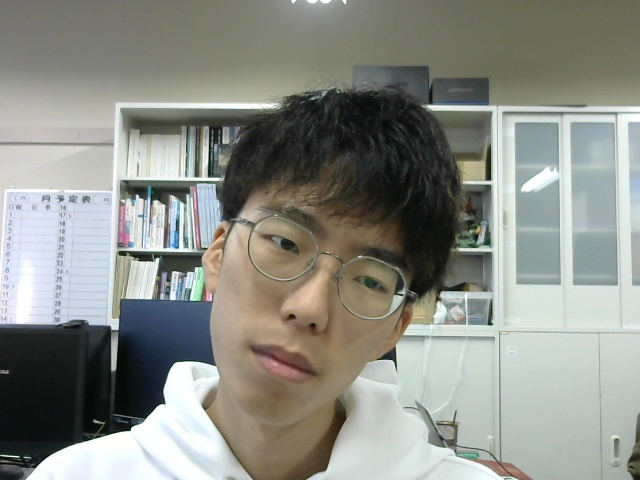
\includegraphics[keepaspectratio, scale=0.08]{figures/texture.jpg}\\
      (a)全方位画像\\
      \\
      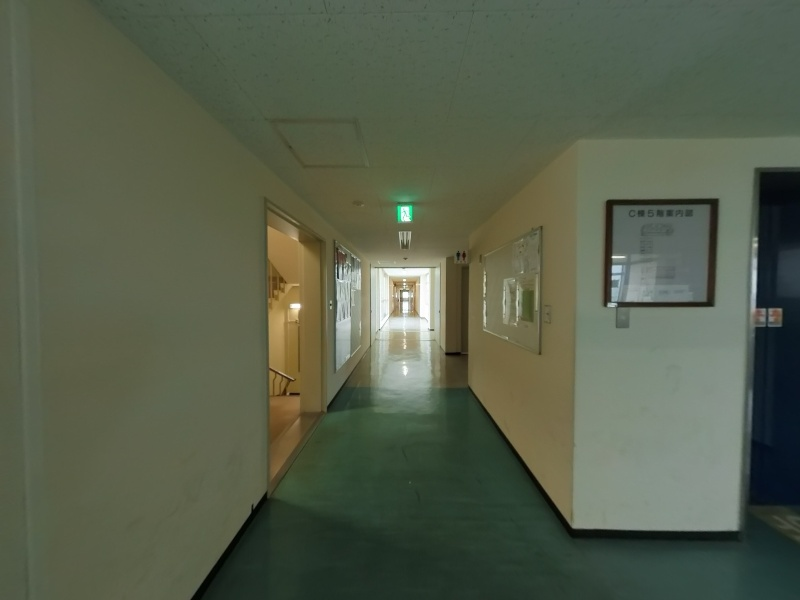
\includegraphics[keepaspectratio, scale=0.4]{figures/output_image.jpg}\\
      (b)透視投影画像\\
    \end{tabular}
  \end{center}
  \caption{出力結果}
  \label{one}
\end{figure}

\section{直行射影の共線性と共面性を用いたカメラ姿勢推定}
直行射影の共線性と共面性を用いたカメラ姿勢推定について簡潔に説明する。
\subsection{直行射影の共線性と共面性}
直行射影の共線性とは直行射影された複数の点が同一直線状に並ぶ性質のことである。
Luらの論文では、カメラ姿勢の反復的最適化を行う際に共線性誤差を検証することで、
カメラ姿勢推定の精度と効率を向上させている。
\\
直行射影の共面性とは射影された複数の点や線が同一平面上に並ぶ性質のことである。
Zhangらの論文では、カメラ姿勢の反復的最適化を行う際に共面性誤差を検証することで、
カメラ姿勢推定の精度と効率を向上させている。
\\
直行射影の共線性を用いた点対応からカメラ姿勢を推定する方法と、直行射影の共面性を用いた線対応からカメラ姿勢を推定する方法は、
直行射影行列が異なるだけである。また、直線の方向ベクトルについても同様に扱うことができるため、
カメラ姿勢を推定するための目的関数を以下のように定義する。
\begin{equation}
  E(\RU,\tU)=\sum^N_{a=1}{||(\IU-\VU_a)(\RU\pU_a+\tU)||}^2+\sum^M_{a=1}{||(\IU-\KU_a)(\RU\rU_a+\tU)||}^2+\sum^M_{a=1}{||(\IU-\KU_a)\RU\dU_a||}^2
\end{equation}
\subsection{カメラ姿勢の推定}
直行射影の共線性と共面性を利用したカメラ姿勢の推定を行う方法を以下に示す。
\subsubsection{入力}
\begin{itemize}
  \item $\pU_a$:世界座標系で表現された空間点の座標
  \item $\vU_a$:$\pU_a$に対応する画像上の特徴点座標
  \item $\dU_a$:世界座標系で表現された直線$L_a$の方向ベクトル
  \item $\rU_a$:世界座標系で表現された直線$L_a$上の点の座標
  \item $\nU_a$:$L_a$に対応する画像上の直線のパラメータベクトル
  \item $\RU^0$:回転行列の初期値
\end{itemize}
\subsubsection{出力}
\begin{itemize}
  \item $\RU$:回転行列
  \item $\tU$:並進ベクトル
\end{itemize}
\subsubsection{アルゴリズム}
1. 共線性拘束のための射影行列を計算する($\vU_a$方向に射影し正規化する) \\ 
\begin{equation}
  \VU_a = \frac{\vU_a\vU_a^\top}{\vU_a^\top\vU_a}
\end{equation}
2. 共面性拘束のための射影行列を計算する($\nU_a$に垂直な方向に射影する) \\
\begin{equation}
  \KU_a = \IU - \nU_a\nU_a^\top
\end{equation}
3. 空間点$\pU_a$を重心$\bar{\pU}$を原点とする座標系で表現する \\
\begin{equation}
  \pU'_a = \pU_a - \bar{\pU}
\end{equation}
4. 空間点$\rU_a$も同様に重心$\bar{\rU}$を原点とする座標系で表現する \\
\begin{equation}
  \rU'_a = \rU_a - \bar{\rU}
\end{equation}
5. $k=0$と初期化する \\
6. 回転行列$\RU^k$を用いて並進ベクトル$\tU$を計算する(式(1)を$t$について変形した形) \\
\begin{equation}
  \tU = \left(\sum^N_{a=1}(\IU-\VU_a)+\sum^N_{a=1}(\IU-\KU_a)\right)^{-1}\left(\sum^N_{a=1}(\VU_a-\IU)\RU^k\pU_a+\sum^N_{a=1}(\KU_a-\IU)\RU^k\rU_a\right)
\end{equation}
7. $\qU_a(\RU^k)$を次のように定義する \\
\begin{equation}
  \qU_a(\RU^k)=\VU_a(\RU^k\pU_a+\tU)
\end{equation}
7. $\sU_a(\RU^k)$を次のように定義する \\
\begin{equation}
  \sU_a(\RU^k)=\KU_a(\RU^k\rU_a+\tU)
\end{equation}
9. 空間点$\qU_a(\RU^k)$を重心$\bar{\qU}$を原点とする座標系で表現する \\
\begin{equation}
  \qU'_a(\RU^k) = \qU_a(\RU^k) - \bar{\pU}
\end{equation}
9. 空間点$\sU_a(\RU^k)$も同様に重心$\bar{\sU}$を原点とする座標系で表現する \\
\begin{equation}
  \sU'_a(\RU^k) = \sU_a(\RU^k) - \bar{\sU}
\end{equation}
10.共分散行列$\MU$を計算する(各群間の分布の主な方向を求める) \\
\begin{equation}
  \MU=\sum^N_{a=1}\qU'_a (\RU^k){\pU'_a}^\top+\sum^M_{a=1}\sU'_a (\RU^k){\rU'_a}^\top+\sum^M_{a=1}(\KU_a\RU^k\dU_a){\dU'_a}^\top
\end{equation}
11.行列$\MU$を特異値分解($\MU=\UU\diag\Sigma\VU^\top$)し、回転行列$\RU^{k+1}$を計算する
\begin{equation}
  \RU^{k+1}=\UU\diag(\sigma,1,\det(\UU\VU^\top))\VU^\top
\end{equation}
12.$||\RU^{k+1}-\RU^k||<\epsilon$であれば、$\RU^{k+1}$に対する$\tU$を式(5)により計算して終了する。
そうでなければ、$k\leftarrow{k+1}$として、ステップ6に戻る

%参考文献
\begin{thebibliography}{99}
\bibitem{bib_1} 菅谷保之,「直交射影の共線性と共面性を用いたカメラ姿勢の推定」
\end{thebibliography}

\end{document}
